\newcommand{\competences}{Alt-C3: Concevoir un algorithme r�pondant � un probl�me pr�cis�ment pos�}

\newcommand{\nom}{Porte conteneur}
\newcommand{\sequence}{03}
\newcommand{\num}{04}
\newcommand{\type}{TD}
\newcommand{\descrip}{Résolution d'un problème en utilisant des méthodes algorithmiques}
\newcommand{\competences}{Alt-C3: Concevoir un algorithme répondant à un problème précisément posé}
\documentclass[10pt,a4paper]{article}
  \usepackage[french]{babel}
  \usepackage[utf8]{inputenc}
  \usepackage[T1]{fontenc}
  \usepackage{xcolor}
  \usepackage[]{graphicx}
  \usepackage{makeidx}
  \usepackage{textcomp}
  \usepackage{amsmath}
  \usepackage{amssymb}
  \usepackage{stmaryrd}
  \usepackage{fancyhdr}
  \usepackage{lettrine}
  \usepackage{calc}
  \usepackage{boxedminipage}
  \usepackage[french,onelanguage, boxruled,linesnumbered]{algorithm2e}
  \usepackage[colorlinks=false,pdftex]{hyperref}
  \usepackage{minted}
  \usepackage{url}
  %\usepackage[locale=FR]{siunitx}
  \usepackage{multicol}
  \makeindex

  %\graphicspath{{../Images/}}

  \renewcommand\listingscaption{Programme}

  %\renewcommand{\thechapter}{\Alph{chapter}}
  \renewcommand{\thesection}{\Roman{section}}
  %\newcommand{\inter}{\vspace{0.5cm}%
  %\noindent }
  %\newcommand{\unite}{\ \textrm}
  \newcommand{\ud}{\mathrm{d}}
  \newcommand{\vect}{\overrightarrow}
  %\newcommand{\ch}{\mathrm{ch}} % cosinus hyperbolique
  %\newcommand{\sh}{\mathrm{sh}} % sinus hyperbolique

  \textwidth 160mm
  \textheight 250mm
  \hoffset=-1.70cm
  \voffset=-1.5cm
  \parindent=0cm

  \pagestyle{fancy}
  \fancyhead[L]{\bfseries {\large PTSI -- Dorian}}
  \fancyhead[C]{\bfseries{{\type} \no \num}}
  \fancyhead[R]{\bfseries{\large Informatique}}
  \fancyfoot[C]{\thepage}
  \fancyfoot[L]{\footnotesize R. Costadoat, J. Genzmer, W. Robert}
  \fancyfoot[R]{\small \today}
  
  \definecolor{bg}{rgb}{0.5,0.5,0.5}
  \definecolor{danger}{RGB}{217,83,79}
  
  \fancypagestyle{correction}{%
  \fancyhf{}
  \lhead{\colorbox{danger}{\begin{minipage}{0.65\paperwidth} \textcolor{white}{\textbf{Correction}} \end{minipage}} }
  \rhead{
\includegraphics[width=2cm]{../../img/logo}}
  \lfoot{Juliette Genzmer, Willie Robert, Renaud Costadoat}
  \rfoot{\colorbox{danger}{\begin{minipage}{0.6\paperwidth} \begin{flushright}\textcolor{white}{\textbf{Correction}}\end{flushright} \end{minipage}} }}

  
  % macro Juliette
  
\usepackage{comment}   
\usepackage{amsthm}  
\theoremstyle{definition}
\newtheorem{exercice}{Exercice}
\newtheorem*{rappel}{Rappel}
\newtheorem*{remark}{Remarque}
\newtheorem*{defn}{Définition}
\newtheorem*{ppe}{Propriété}
\newtheorem{solution}{Solution}


\section{Pr�sentation de la probl�matique}

\begin{minipage}{0.45\linewidth}
L'objectif est d'usiner une pi�ce dont les caract�ristiques sont repr�sent�es sur la g�om�trie ci-jointe. Pour cela il est n�cessaire de d�terminer une trajectoire d'usinage qui convient.
\end{minipage}\hfill
\begin{minipage}{0.45\linewidth}
\begin{center}
 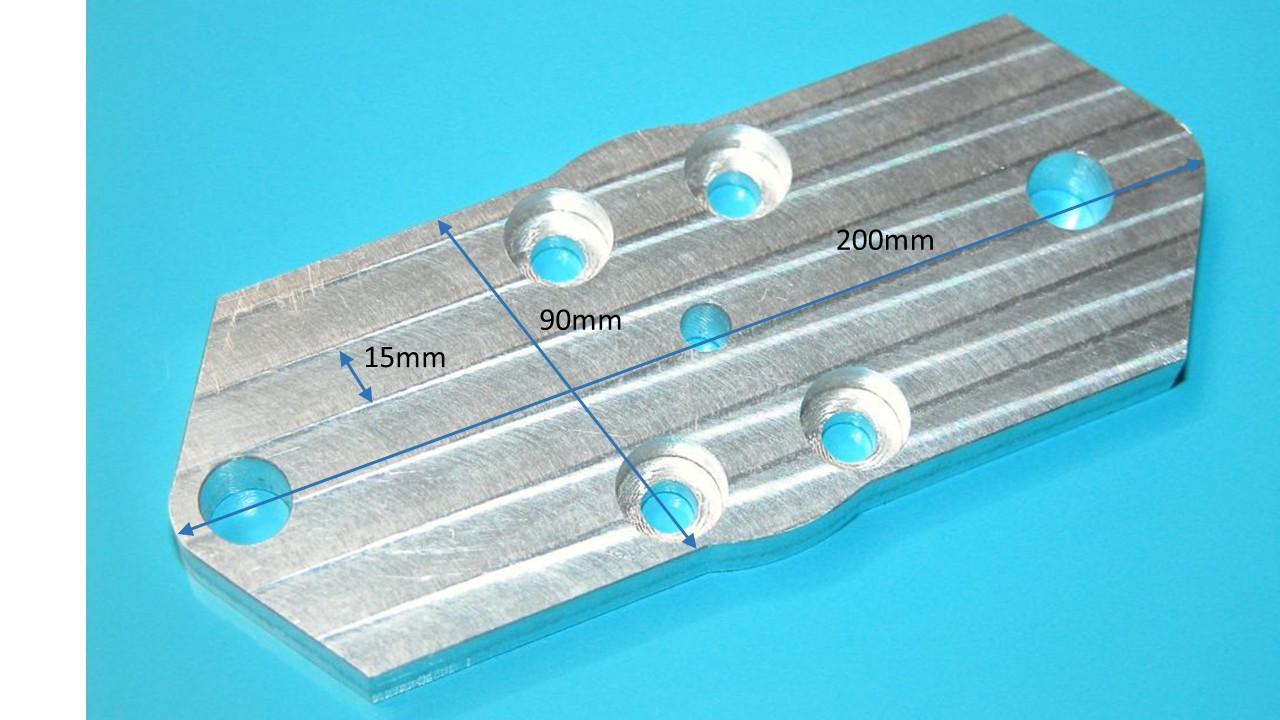
\includegraphics[width=0.8\linewidth]{img/fig1.png}
\end{center}
\end{minipage}

~\

La trajectoire sera r�pr�sent�e sous la forme de deux listes de coordonn�es \verb? x,y ?.

\section{Programmation de la trajectoire}

\paragraph{Question 1:} Proposer une fonction \verb? ligne_droite(x,y,Lx,Ly,n)? dont les donn�es d'entr�e sont:
\begin{itemize}
 \item \verb? x,y ?: les listes de coordonn�es ,
 \item \verb? Lx,Ly ?: les longueurs des d�placements sur $x$ et $y$,
 \item \verb? n ?: le nombre d'�tapes du d�placement.
\end{itemize}

\paragraph{Question 2:} Proposer une fonction \verb? tourner()? ou deux fonctions \verb? tourner_a_gauche()? et \verb? tourner_a_droite()? qui permettent � l'outil d'effectuer les trajectoires circulaires n�cessaires pour compl�ter la trajectoire. Il faudra utiliser le minimum de fonction possible.

\paragraph{Question 3:} Proposer un code utilisant les fonctions pr�c�dentes permettant d'effectuer la trajectoire suivante. Le code permettant de tracer le rectangle image de la pi�ce est donn�e.

\begin{minipage}{0.55\linewidth}
\begin{GrayBox}[0.85\textwidth]
\small\begin{verbatimtab}[3]
import matplotlib.pyplot as plt
from matplotlib.patches import Rectangle

someX, someY = 0, 0
plt.figure()
currentAxis = plt.gca()
currentAxis.add_patch(Rectangle((
	someX - .1, someY - .1), 90, 
	200,alpha=1, facecolor='grey'))
plt.plot(x, y)
plt.axis([-20, 120, -40, 240])
plt.show()
\end{verbatimtab}
\end{GrayBox}
\end{minipage}\hfill
\begin{minipage}{0.4\linewidth}
\begin{center}
 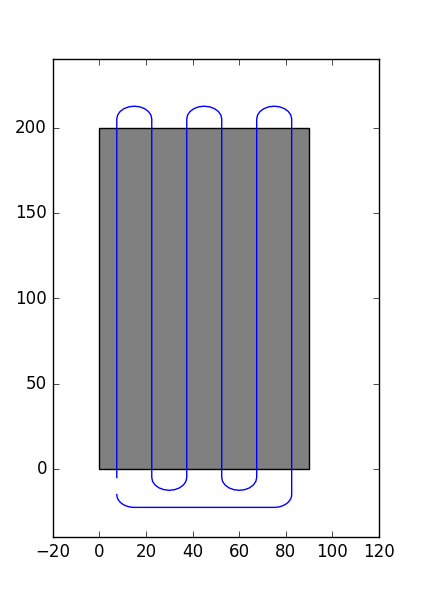
\includegraphics[width=0.8\linewidth]{img/fig2.png}
\end{center}
\end{minipage}

\end{document}
